%%%%%%%%%%%%%%%%%%%%%%%%%%%%%%%%%%%%%%%%%
% University of Hong Kong Masters/Doctoral Thesis 
% LaTeX Template
% Version 3.1 (28/03/2023)
% 
% Version 3 modification by:
% Nan Meng (u3003637@connect.hku.hk)
%
% Version 2.x major modifications by:
% Vel (vel@latextemplates.com)
% 
% This template is based on the template by:
% Steve Gunn (http://users.ecs.soton.ac.uk/srg/softwaretools/document/templates/)
% Sunil Patel (http://www.sunilpatel.co.uk/thesis-template/)
% Johannes Böttcher (http://www.latextemplates.com/template/masters-doctoral-thesis)
%
% Template license:
% CC BY-NC-ND 4.0 (https://creativecommons.org/licenses/by-nc-nd/4.0/)
%
% Author:  Lei XIA
% Contact: brianleixia@connect.hku.hk
%
%%%%%%%%%%%%%%%%%%%%%%%%%%%%%%%%%%%%%%%%%


%----------------------------------------------------------------------------------------
%	PACKAGES AND OTHER DOCUMENT CONFIGURATIONS
%----------------------------------------------------------------------------------------

\documentclass[
12pt, % The default document font size, options: 10pt, 11pt, 12pt
%oneside, % Two side (alternating margins) for binding by default, uncomment to switch to one side
english, % ngerman for German
onehalfspacing, % Single line spacing (singlespacing), alternatives: onehalfspacing or doublespacing
% draft, % Uncomment to enable draft mode (no pictures, no links, overfull hboxes indicated)
% nolistspacing, % If the document is onehalfspacing or doublespacing, uncomment this to set spacing in lists to single
liststotoc, % Uncomment to add the list of figures/tables/etc to the table of contents
%toctotoc, % Uncomment to add the main table of contents to the table of contents
parskip, % Uncomment to add space between paragraphs
%nohyperref, % Uncomment to not load the hyperref package
headsepline, % Uncomment to get a line under the header
chapterinoneline, % Uncomment to place the chapter title next to the number on one line
openany
%consistentlayout, % Uncomment to change the layout of the declaration, abstract and acknowledgements pages to match the default layout
]{HKUThesis} % The class file specifying the document structure

\usepackage[utf8]{inputenc} % Required for inputting international characters
\usepackage[T1]{fontenc} % Output font encoding for international characters
\usepackage{fontawesome} % Awesome symbol for usage
\usepackage{wrapfig} % Add enbedded figure in the text
\usepackage{tikz} % Add the signature figure overlap the text
% \usepackage[labelformat=simple]{subcaption} % Add multiple subfigures in a figure environment
% \captionsetup{justification=justified, margin=0pt}
% \renewcommand\thesubfigure{(\Alph{subfigure})} % change the image numbering and reference link to (A),(B),(C), ...... format

\usepackage{mathpazo} % Use the Palatino font by default
%\usepackage[backend=bibtex,style=alphabetic,natbib=true]{biblatex} % Use the bibtex backend with the authoryear citation style (which resembles APA)
\usepackage[natbib=true,maxbibnames=99,firstinits=true]{biblatex}

\addbibresource{thesis.bib} % The filename of the bibliography

\usepackage[autostyle=true]{csquotes} % Required to generate language-dependent quotes in the bibliography

\AtBeginEnvironment{enquote}{\itshape} % change the quote words to italics style

\usepackage{rotating} % Required to add rotated big tables

\usepackage[normalem]{ulem} % Required to add dashed underlines

\setlength\parindent{2em}
%----------------------------------------------------------------------------------------
%	MARGIN SETTINGS
%----------------------------------------------------------------------------------------

\geometry{
	paper=a4paper, % Change to letterpaper for US letter
	left=28mm, % Left margin
	right=29mm, % Right margin
	bindingoffset=.5cm, % Binding offset
	top=2.5cm, % Top margin
	bottom=2.5cm, % Bottom margin
	%showframe, % Uncomment to show how the type block is set on the page
}

% Times New Roman font setup
\usepackage{times} % Uncomment this to use Times New Roman font
\usepackage{mathptmx}

\RenewDocumentCommand{\abovechapterskip}{}{\vspace*{-20pt}} % 减小章节标题上方的空间


%----------------------------------------------------------------------------------------
%	THESIS INFORMATION
%----------------------------------------------------------------------------------------

\thesistitle{Topic Guided Multi-faceted Semantic Disentanglement for CTR prediction}
% Thesis title, this is used in the title and abstract, print it elsewhere with \ttitle

\supervisor{Prof. FirstName \textsc{FamilyName}}
% Your supervisor's name, this is used in the title page, print it elsewhere with \supname

\cosupervisor{Prof. FirstName \textsc{FamilyName}}
% Your supervisor's name, this is used in the title page, print it elsewhere with \supname
% \cosupervisor{Prof. Hayden K.-H. \textsc{So}} % Your supervisor's name, this is used in the title page, print it elsewhere with \cosupname

\examiner{}
% Your examiner's name, this is not currently used anywhere in the template, print it elsewhere with \examname

\degree{Master of Science}
% Your degree name, this is used in the title page and abstract, print it elsewhere with \degreename

\author{Lei \textsc{Xia}}
% The author name, this is used in the title page and abstract, print it elsewhere with \authorname

\addresses{}
% Your address, this is not currently used anywhere in the template, print it elsewhere with \addressname

\subject{Natural Language Processing}
% Your subject area, this is not currently used anywhere in the template, print it elsewhere with \subjectname

\keywords{pre-trained language model, large language processing, supervised fine-tuning}
% Keywords for your thesis, this is not currently used anywhere in the template, print it elsewhere with \keywordnames

\university{University of Hong Kong}
% Your University's name and URL, this is used in the cover page and abstract, print it elsewhere with \univname

\bsuniversity{HKU}
\msuniversity{HKU}
% Your Bachelor/Master University's name and URL, this is used in the title page and abstract, print it elsewhere with \univname

\department{Department of Computer Science}
% Your department's name and URL, this is used in the title page and abstract, print it elsewhere with \deptname

\group{Laboratory of The Student}
% Your research group's name and URL, this is used in the title page, print it elsewhere with \groupname

\faculty{School of Computing and Data Science}
% Your faculty's name and URL, this is used in the title page and abstract, print it elsewhere with \facname

\AtBeginDocument{
\hypersetup{pdftitle=\ttitle} % Set the PDF's title to your title
\hypersetup{pdfauthor=\authorname} % Set the PDF's author to your name
\hypersetup{pdfkeywords=\keywordnames} % Set the PDF's keywords to your keywords
}
% \AtBeginEnvironment{algorithm}{\setstretch{2}}
\setlength{\algomargin}{1.3ex}


%----------------------------------------------------------------------------------------
%	NEW COMMAND DEFINITION
%----------------------------------------------------------------------------------------
\newcommand{\codestyle}[1]{\colorbox{gray!20}{\darkred{#1}}}

% ======================================================================================== %
%                                        START DOCUMENT
% ======================================================================================== %

\begin{document}

\frontmatter % Use roman page numbering style (i, ii, iii, iv...) for the pre-content pages
\pagestyle{plain} % Default to the plain heading style until the thesis style is called for the body content


%----------------------------------------------------------------------------------------
%	COVER
%----------------------------------------------------------------------------------------

\begin{titlepage}
\addtocounter{page}{-1}
\begin{center}

% \vspace*{.024\textheight}
\begin{center}
    
\includegraphics[width=0.3\textwidth]{Covers/hkulogo.png} % Include the university logo image
\end{center}

% \vspace{0.5cm}
% \textsc{\Large Doctoral Thesis}\\[0.5cm] % Thesis type
\vspace{40pt} % Add some vertical spacing

% University details
\begin{center}
    {The University of Hong Kong}\\[10pt] % University name
    {School of Computing and Data Science}\\[10pt] % Faculty name
    {Department of Computer Science}\\[25pt] % Department name
\end{center}

% \rule[0.4cm]{13cm}{0.1pt}\\% \HRule \\[0.4cm] % Horizontal line
% {\huge \bfseries \ttitle\par}\vspace{0.4cm} % Thesis title
% % \HRule \\[1.5cm] % Horizontal line
% \rule{13cm}{0.1pt}\\ \vspace{1.5cm}
 
% \begin{minipage}[t]{0.4\textwidth}
% \begin{flushleft} \large
% \emph{Author:}\\
% \href{http://#}{\authorname} % Author name - remove the \href bracket to remove the link
% \end{flushleft}
% \end{minipage}
% \begin{minipage}[t]{0.4\textwidth}
% \begin{flushright} \large
% \emph{Supervisor:} \\
% \href{https://www.eee.hku.hk/~elam/}{\supname} \\ % Supervisor name - remove the \href bracket to remove the link
% \emph{Co-Supervisor:} \\
% \href{https://www.eee.hku.hk/~hso/}{\cosupname} % Supervisor name - remove the \href bracket to remove the link 
% \end{flushright}
% \end{minipage}\\[1.6cm]

\vspace{30pt} % Add some vertical spacing
% Course code and dissertation title
\begin{center}
    {COMP7704}\\[10pt] % Course code
    {Dissertation Title}\\ % Dissertation title placeholder
    {Topic Guided Multi-faceted Semantic Disentanglement for CTR prediction}\\[20pt] % Placeholder for the actual title
\end{center}

\vspace{40pt} % Add some vertical spacing

% \large \textit{A thesis submitted in fulfillment of the requirements\\ for the degree of \degreename}\\[0.3cm] % University requirement text
% \textit{in the}\\[0.4cm]
% % \groupname\\
% \deptname\\\facname\\[1.6cm] % Research group name and department name

% Submission details
\begin{center}
    {Submitted in partial fulfillment of the requirements for the admission to\\
    the degree of Master of Science in Computer Science}\\[20pt]
\end{center}

\vspace{20pt} % Add some vertical spacing

% {\large \usdate\today}\\[4cm] % Date
%\includegraphics{Logo} % University/department logo - uncomment to place it

% Author and supervisor details
\begin{center}
    {By\\
    \textbf{\textsc{Bai} Junhao}  ({UID: 3036382909})\\[10pt] 
    \textbf{\textsc{Long} Qian}   ({UID: 3036380559})\\[10pt]
    \textbf{\textsc{Yin} Zhiqian} ({UID: 3036380298})\\[10pt] 
    
    Supervisor: Prof. H.F. Ting\\ % Replace with the supervisor's title and name
    Date of submission: 2025/07/18} % Replace with the submission date
\end{center}

\vfill
\end{center}

\end{titlepage}


% \blankpage
% \addtocounter{page}{-1}


%----------------------------------------------------------------------------------------
%	ABSTRACT PAGE
%----------------------------------------------------------------------------------------


\begin{abstract}
\addchaptertocentry{\abstractname} % Add the abstract to the table of contents
Put Your \emph{Abstract} Here ...

\bigskip
\noindent This latex project is a doctoral thesis template for the University of Hong Kong. The style and design of the entire project closely follow the official guidelines from the Graduate School: \href{https://intraweb.hku.hk/reserved_1/gradsch/PreparingandSubmittingYourThesis.pdf}{\textbf{Preparing and Submitting Your Thesis --- A Guide for MPhil and PhD Students.}} Generally, there is no strict stipulations on the style or format of different components of the thesis, except for the \textbf{Abstract}. According to the detailed regulations [\href{https://intraweb.hku.hk/reserved_1/gradsch/regulations_procedures/format_binding_presentation.pdf}{\textbf{Link}}], the \textbf{Abstract} should be part of the thesis with \uline{no fewer than 200 and no more than 500 words}. The format shall be the same as that of the thesis itself. The front page of each abstract shall contain the statement which includes:
\begin{itemize}
    \item Abstract of thesis entitled ``\dotuline{\hspace{8cm}}''
    \item Submitted by \dotuline{\hspace{10cm}}~
    \item for the degree of \dotuline{\hspace{9.5cm}}~
    \item at the \univname~in (\usdate\today).
\end{itemize}

In addition to the opening of abstract, the abstract \uline{should appear before the title page}. The abstract in this template is \uline{not numbered, or counted in the pagination of the front matter, or listed in the table of contents}. All the requirements are fulfilled in this template.



\end{abstract}


%----------------------------------------------------------------------------------------
%	TITLE PAGE
%----------------------------------------------------------------------------------------
% \pagestyle{empty}
\newpage
\addtocounter{page}{-1}
\begin{center}
\vspace*{2cm}
\huge{ \bf \ttitle}
\end{center}

\vspace{20mm}
\begin{center}
by

\vspace{10mm}
{\bf \authorname}\\
B.S. \textit{\bsunivname} M.S. \textit{\msunivname}
\end{center}

\vspace{30mm}
\begin{center}
A Thesis Submitted in Partial Fulfilment \\
of the Requirements for the Degree of \\
Doctor of Philosophy \\
\vspace{10mm}
at \\
\vspace{10mm}
\univname\\
%February 2015
\monthyeardate\today
\end{center}

%----------------------------------------------------------------------------------------
%	COPYRIGHT PAGE
%----------------------------------------------------------------------------------------

% \newpage
\thispagestyle{empty}
\addtocounter{page}{-1}
\vspace*{\fill}
\scshape \noindent Copyright \copyright 2020, by \authorname \\
\noindent all rights reserved.
\vspace*{\fill}
\newpage
\rm


%----------------------------------------------------------------------------------------
%	DECLARATION PAGE
%----------------------------------------------------------------------------------------

\begin{declaration}
\setcounter{page}{1}
\addchaptertocentry{\authorshipname} % Add the declaration to the table of contents

\vspace{0.6cm}
I, \authorname, declare that this dissertation titled, \enquote{\ttitle}, which is submitted in fulfillment of the requirements for the Degree of Master of Science, represents my own work except where due acknowledgement have been made. I further declared that it has not been previously included in a thesis, dissertation, or report submitted to this University or to any other institution for a degree, diploma or other qualifications.


\vspace{2cm} 
\begin{flushright}
\hfill Signed: \underline{\hspace{5cm}}\\[2em] % This prints a line for the signature
\hfill Date: \underline{\hspace{1.5cm} \usdate\today \hspace{1.5cm}}\\ % This prints a line to write the date
\end{flushright}

% Signature
\begin{tikzpicture}[remember picture,overlay]
\node[xshift=-6cm,yshift=-18cm] at (current page.north east){%
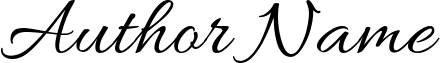
\includegraphics[width=3.6cm]{Figures/signature.png}};
\end{tikzpicture}
\end{declaration}





%----------------------------------------------------------------------------------------
%	QUOTATION PAGE
%----------------------------------------------------------------------------------------

% \newpage
\thispagestyle{empty}
\vspace*{\fill}
\begin{center}
% Font family: ''Calling Angels Personal Use'' from website https://www.dafont.com

\includegraphics[width=0.8\textwidth]{Dedication/dedication.pdf}
\end{center}
\vspace*{\fill}



%----------------------------------------------------------------------------------------
%	ACKNOWLEDGEMENTS
%----------------------------------------------------------------------------------------
\begin{acknowledgements}
\setcounter{page}{2}
\addchaptertocentry{\acknowledgementname} % Add the acknowledgements to the table of contents
\vspace{1cm}


\noindent We would like to thank our supervisor, Professor H.F. Ting, for his guidance and support during the course of this research.
\\[0.4cm]

% \hfill
\begin{flushright}
    \authorname \\
    The University of Hong Kong \\
    \usdate\today
\end{flushright}

\end{acknowledgements}

%----------------------------------------------------------------------------------------
%	LIST OF PUBLICATIONS PAGES
%----------------------------------------------------------------------------------------
% \begin{publications}
\addcontentsline{toc}{chapter}{List of Publications}
\newcommand{\JourConfTitle}[1]{\ul{\emph{#1}}}

% ---------------------------------------------------------------------------
% JOURNALS
% ---------------------------------------------------------------------------

\begin{journals}
\item \textbf{Nan Meng}, Hayden K.-H. So, Xing Sun, and Edmund Y. Lam, ``High-dimens-ional dense residual convolutional neural network for light field reconstruction,'' \JourConfTitle{IEEE Transactions on Pattern Analysis and Machine Intelligence}, October 2019.

\item \textbf{Nan Meng}, Zhou Ge, Tianjiao Zeng, and Edmund Y. Lam, ``LightGAN: a deep generative model for light field reconstruction,'' \JourConfTitle{IEEE Access}, June 2020.

\item \textbf{Nan Meng}, Xing Sun, Hayden K.-H. So, and Edmund Y. Lam, ``Computational light field generation using deep nonparametric Bayesian learning,'' \JourConfTitle{IEEE Access}, vol. 7, pp. 24990--25000, February 2019.

\item \textbf{Nan Meng}, Edmund Y. Lam, Kevin K.-M. Tsia and Hayden K.-H. So, ``Large-scale multi-class image-based cell classification with deep learning,'' \JourConfTitle{IEEE Journal of Biomedical and Health Informatics}, vol. 23, no. 5, pp. 2091--2098, September 2019. 
\end{journals}

% \newpage
% ---------------------------------------------------------------------------
%  CONFERENCES
% ---------------------------------------------------------------------------

\begin{conferences}
\item \textbf{Nan Meng}, Xiaofei Wu, Jianzhuang Liu, and Edmund Y. Lam, ``High-order residual network for light field super-resolution,'' in \JourConfTitle{Association for the Advancement of Artificial Intelligence}, vol. 34, no.7, pp. 11757-11764, 2020.

\item \textbf{Nan Meng}, Tianjiao Zeng, and Edmund Y. Lam, ``Spatial and angular reconstruction of light field based on deep generative networks,'' in \JourConfTitle{IEEE International Conference on Image Processing}, pp. 4659–4663, September 2019.

\item \textbf{Nan Meng}, Tianjiao Zeng, and Edmund Y. Lam, ``Perceptual loss for light field reconstruction in high-dimensional convolutional neural networks,'' in \JourConfTitle{OSA Topical Meeting in Computational Optical Sensing and Imaging}, pp. CW1A.5, June 2019.

\item Edmund Y. Lam, \textbf{Nan Meng}, and Hayden K.H. So, ``Deep convolutional neural network for single-cell image analysis,'' in \JourConfTitle{High-Speed Biomedical Imaging and Spectroscopy: Toward Big Data Instrumentation and Management}, volume 10505 of Proceedings of the SPIE, pp. 105050K, January 2018.

\item \textbf{Nan Meng}, Hayden K.-H. So, and Edmund Y. Lam, ``Computational single-cell classification using deep learning on bright-field and phase images,'' in \JourConfTitle{IAPR Conference on Machine Vision Applications}, pp. 164–167, May 2017.

\item Xing Sun, Zhimin Xu, \textbf{Nan Meng}, Edmund Y. Lam, and Hayden K.-H. So, ``Data-driven light field depth estimation using deep convolutional neural networks,'' in \JourConfTitle{IEEE International Joint Conference on Neural Networks}, pp. 367–374, July 2016.

\item Xing Sun, \textbf{Nan Meng}, Zhimin Xu, Edmund Y. Lam, and Hayden K.-H. So, ``Sparse hierarchical nonparametric Bayesian learning for light field representation and denoising,'' in \JourConfTitle{IEEE International Joint Conference on Neural Networks}, pp. 3272–3279, July 2016.
\end{conferences}

\begin{patents}
\item \textbf{Nan Meng}, Xiaofei Wu, Jianzhuang Liu, ``Image Enhancement and Reconstruction based on Camera Array'', [\emph{under review}]
\end{patents}

\begin{datasets}
\item \textbf{Nan Meng}, Edmund Lam, Tsia, Kevin Kin Man, So, Hayden Kwok-Hay, ``Human somatic label-free bright-field cell images'', IEEE Dataport, 2018. [\darkred{Online}]. Available: \url{http://dx.doi.org/10.21227/H2QW97}. Accessed: Mar. 13, 2019.
\end{datasets}

\end{publications}


%----------------------------------------------------------------------------------------
%	LIST OF CONTENTS/FIGURES/TABLES PAGES
%----------------------------------------------------------------------------------------

\tableofcontents % Prints the main table of contents

\listoffigures % Prints the list of figures

\listoftables % Prints the list of tables

% \listofalgorithms % Prints the list of algorithms
% \addchaptertocentry{\listalgorithmcfname}
%----------------------------------------------------------------------------------------
%	ABBREVIATIONS
%----------------------------------------------------------------------------------------
% \begin{abbreviations}{ll} % Include a list of abbreviations (a table of two columns)

\textbf{ASAP} & \textbf{A}s \textbf{S}oon \textbf{A}s \textbf{P}ossible \\
\textbf{AKA} & \textbf{A}lso \textbf{K}nown \textbf{A}s \\
\textbf{BPFA} & \textbf{B}eta \textbf{P}rocess \textbf{F}actor \textbf{A}nalysis \\
\textbf{CNN} & \textbf{C}onvolutional \textbf{N}eural \textbf{N}etwork \\
\textbf{GAN} & \textbf{G}enerative \textbf{A}dversarial \textbf{N}etwork \\
\textbf{MSE} & \textbf{M}ean \textbf{S}quare \textbf{E}rror \\
\textbf{PSNR} & \textbf{P}eak \textbf{S}ignal-to-\textbf{N}oise \textbf{R}atio \\
\textbf{SSIM} & \textbf{S}tructural \textbf{SIM}ilarity \\

\end{abbreviations}


%----------------------------------------------------------------------------------------
%	SYMBOLS
%----------------------------------------------------------------------------------------
% \begin{symbols}{p{0.15\textwidth}p{0.7\textwidth}l} % Include a list of Symbols (a three column table)

\multicolumn{3}{l}{\symboltitle{Global notations}}\\ \\
$I^\mathrm{SR}$ & super-resolved light field image & --- \\
$I^\mathrm{LR}$ & low-resolution light field image & --- \\
$I^\mathrm{HR}$ & high-resolution light field image & --- \\
$E^\mathrm{SR}$ & super-resolved epipolar plane image & --- \\
$E^\mathrm{HR}$ & high-resolution epipolar plane image & --- \\ \\
% $L$ & light field function & --- \\

\multicolumn{3}{l}{\symboltitle{Chapter~1}}\\ \\
$\theta$, $\phi$ & incoming direction expressed in term of spherical coordinates & rad \\
$\tau$ & time & s (second)\\
$x$,$y$ & spatial coordinates with two-plane parameterization & 1 (uint) \\
$s$,$t$ & angular coordinates with two-plane parameterization & 1 (uint) \\
$P$ & radiance distribution & \si{\watt\per\steradian \square{\metre} \text{\hertz}} \\
$\Omega$ & image plane & --- \\
$\Theta$ & parameters of the multi-layer framework & --- \\
$\gamma_s$, $\gamma_a$ & scaling factors of spatial / angular coordinates & 1 (uint) \\
$\mathcal{L}$ & loss function & --- \\ \\

\multicolumn{3}{l}{\symboltitle{Chapter~2}}\\ \\
$F_0$ & shallow features extracted by a single HConv layer & --- \\
$F_\mathrm{G_d}$ & feature maps extracted by the $d^\mathrm{th}$ HRB of the GRLNet & --- \\
$H_\mathrm{HRB}^\mathrm{n}$ & the operation of the $n^\mathrm{th}$ HRB of the SReNet & --- \\
$H_\mathrm{AGBN}$ & the operation of the proposed aperture group batch normalization algorithm & --- \\
$H_\mathrm{up}$ & upsampling operation on the low-resolution features & --- \\ \\


$\ell_A$ & angular loss & --- \\
$\ell_S$ & spatial perceptual loss & --- \\ 
$\ell_{SA}$ & the weighted combination of $\ell_A$ and $\ell_S$& --- \\
$f$ & the summation of all the feature maps after every activation function of VGG network & --- \\
$g$ & learned mapping between the low-resolution and high-resolution light field images & --- \\ \\


\multicolumn{3}{l}{\symboltitle{Chapter~3}}\\ \\
$x$,$y$ & spatial coordinates with two-plane parameterization & 1 (uint) \\
$s$,$t$ & angular coordinates with two-plane parameterization & 1 (uint) \\
$\gamma_s$, $\gamma_a$ & scaling factors of spatial / angular coordinates & 1 (uint) \\
$\ell_G$ & generator adversarial loss & --- \\
$\phi$ & denotes the mapping of VGG network & --- \\
$\delta$ & nearest neighbor downsampling operator & --- \\
$\kappa$ & a Gaussian blurring kernel with a window size of $7 \times 7$ and standard deviation of 1.2 pixels & --- \\
$\eta$ & additive noise with zero mean and unit standard deviation & --- \\ \\

\end{symbols}


%----------------------------------------------------------------------------------------
%	THESIS CONTENT - CHAPTERS
%----------------------------------------------------------------------------------------

\mainmatter % Begin numeric (1,2,3...) page numbering

\pagestyle{thesis} % Return the page headers back to the "thesis" style

% Include the chapters of the thesis as separate files from the Chapters folder
% Uncomment the lines as you write the chapters

\chapter{Introduction}

\label{chap:introduction}

Click-through rate (CTR) prediction lies at the heart of the online advertising ecosystem and recommendation systems, aiming to estimate a user’s likelihood of clicking on a specific item or advertisement. Accurate CTR predictions enable service providers to generate more relevant and diverse recommendation lists, thereby improving user experience, engagement, and platform revenue. Consequently, CTR prediction has garnered significant attention from both industry professionals and academic researchers.

\begin{figure}[t]
    \centering
    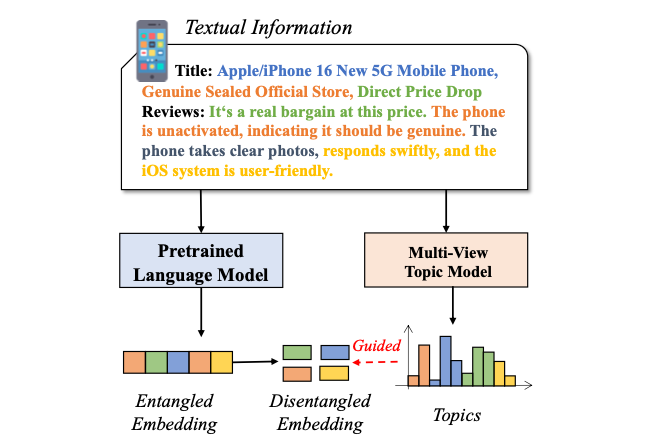
\includegraphics[width=0.9\linewidth]{Figures/Chapter1/figure1.png}
    \caption{Illustration of semantic embedding disentanglement.}
    \label{fig:disentangle}
\end{figure}

Conventional CTR prediction methods typically comprise four main layers: the input layer, embedding layer, interaction layer, and prediction layer. The input layer incorporates a variety of features, including user attributes (e.g., gender, age, occupation, behavior sequences), item characteristics (e.g., category, brand), and contextual information (e.g., interaction location, time). These features are initially processed through the embedding layer to obtain feature embeddings. Subsequently, feature interaction layers, such as Factorization Machines, EulerNet, or KAN, conduct interactions on the feature embeddings. The resulting interacted features are then fed into the prediction layer to estimate the final click probability.

Traditional CTR models primarily rely on structured categorical and numerical features. However, with the rapid advancement of Pretrained Language Models (PLMs), researchers have begun incorporating textual information to enrich semantic understanding and improve prediction accuracy. For instance, CTRL collects textual descriptions of features and encodes them using PLMs to derive semantic embeddings. It employs a contrastive learning strategy to align collaborative signals with these semantic embeddings. Despite the effectiveness of PLMs in extracting semantic features, existing methods typically encode all textual information into a single dense embedding. As illustrated in Figure~\ref{fig:disentangle}, since textual descriptions inherently contain multiple aspects—such as brand, price, quality, and user sentiment—compressing them into a single representation leads to an entangled embedding. This entanglement hinders fine-grained feature interactions, limiting the model’s ability to distinguish between different aspects of user preferences.

Addressing this issue presents two major challenges: 
(1) How can we effectively disentangle and extract meaningful knowledge from textual information? Text descriptions contain rich but interwoven semantic aspects, making it challenging to separate distinct information (e.g., product features, user sentiment, and brand identity) and filter out noise. 
(2) How can we effectively integrate multi-faceted knowledge into the CTR prediction task to extract useful information? Not all extracted textual information is relevant to user decision-making, so aligning it with CTR prediction is crucial for performance improvement.

To address these challenges, we propose \textbf{Multi-faceted Semantic Disentanglement for CTR prediction (MSD-CTR)}. MSD-CTR consists of two components: 
\begin{itemize}
    \item \textbf{Disentangled Semantic Topic Model (DSTopic)} employs a disentangled generative process to capture different aspects of documents using a Disentangled Semantic VAE (DSVAE) and a vocabulary clustering module.
    \item \textbf{Topic Guided Disentangled Representation Learning (TopicDRL)} incorporates the multi-faceted knowledge into CTR prediction, introducing an individual-level alignment loss and an intra-view contrastive loss to guide semantic embedding learning.
\end{itemize}

To evaluate the performance of MSD-CTR, we conduct extensive experiments on four real-world datasets and implement our model based on two foundational CTR methods. The results demonstrate that MSD-CTR outperforms existing CTR models. Additionally, we perform ablation studies and qualitative analyses to validate the effectiveness of the proposed components.

\textbf{Our contributions can be summarized as follows:}
\begin{enumerate}
    \item We investigate text-enhanced CTR methods and analyze the issue of entangled semantic embeddings.
    \item We propose MSD-CTR, a novel framework that disentangles and incorporates multi-faceted knowledge from textual information via DSTopic and TopicDRL modules.
    \item We conduct extensive experiments demonstrating the superior performance of MSD-CTR and validate the contributions of its individual components.
\end{enumerate}



\chapter{Preliminary}

\section{Problem Definition}

Click-through rate (CTR) prediction is a binary classification task. The conventional CTR prediction dataset $\mathcal{D}$ consists of $N$ samples, each represented as a pair $(\mathbf{x}_i, y_i)$, where the label $y_i \in \{0, 1\}$ indicates the user’s click behavior (1 for click, 0 for no click). The input instance is denoted by $\mathbf{x}_i = \{x_{i,1}, x_{i,2}, \cdots, x_{i,m}\}$, where $m$ represents the number of feature fields, and each feature $x_{i,m}$ is a high-dimensional one-hot vector.

In traditional CTR scenarios, a $D$-dimensional embedding layer $\mathcal{E} = \{E_1, E_2, \cdots, E_m\}$ maps the high-dimensional sparse vector $\mathbf{x}_i$ into a low-dimensional dense embedding $\mathbf{e}_i = \{e_{i,1}, e_{i,2}, \cdots, e_{i,m}\}$, where $e_{i,m} \in \mathbb{R}^{D}$, which is more suitable for learning in deep models. The CTR prediction model $f_{\text{CTR}}$ then estimates the click probability $y_i$ based on these embeddings, formulated as:
\[
y_i = f_{\text{CTR}}(e_{i,1}, e_{i,2}, \cdots, e_{i,m}).
\]

\textbf{Text-enhanced CTR prediction:} With the advent of Pretrained Language Models (PLMs), some studies have attempted to incorporate textual information into CTR prediction. Let $t_i$ denote the textual information associated with the sample $(\mathbf{x}_i, y_i)$, which may include the item title, description, and reviews. This textual information is typically encoded by a PLM, formulated as:
\[
\mathbf{t}_i = f_{\text{PLM}}(t_i), \quad \mathbf{t}_i \in \mathbb{R}^{D_{\text{PLM}}},
\]
where $D_{\text{PLM}}$ denotes the dimension of the PLM embedding. The semantic embedding $\mathbf{t}_i$ is then integrated into the CTR model to enhance prediction performance:
\[
y_i = f_{\text{CTR}}(f_{\text{text}}(\mathbf{t}_i), e_{i,1}, e_{i,2}, \cdots, e_{i,m}),
\]
where $f_{\text{text}}$ is a fully connected network that aligns the embedding size to facilitate feature interactions.

Due to the rich information in $t_i$, the encoded semantic embedding $\mathbf{t}_i$ often captures multiple latent aspects, leading to an entangled representation. In this study, we focus on disentangling the entangled semantic embedding $\mathbf{t}_i$ into distinct, meaningful embeddings to enhance interpretability and effectiveness.

\section{Topic Model}

To perform the disentangling task, we employ topic modeling to capture distinct semantic aspects from textual information. A topic model is a statistical approach for discovering hidden semantic structures in a collection of documents. In this study, we treat the textual information of all items as a document corpus, denoted as $\mathcal{T} = \{t_j \mid j \in [1, 2, \cdots, J]\}$, where $J$ is the total number of items. Each document $t_j$ is represented as a Bag-of-Words (BoW) vector $\mathbf{b}_j \in \mathbb{R}^{V}$, where $V$ is the vocabulary size.

The topic model assumes that each document is generated from a mixture of topics (document’s topic distribution), where each topic is characterized by a distribution over words (topic-word distribution). ETM factorizes the topic-word distribution into a topic embedding matrix $\alpha \in \mathbb{R}^{K \times D_{\text{TM}}}$ and a word embedding matrix $\rho \in \mathbb{R}^{V \times D_{\text{TM}}}$, where $K$ is the number of topics and $D_{\text{TM}}$ is the dimensionality of the embeddings. The topic-word distribution matrix $\beta \in \mathbb{R}^{K \times V}$ is computed as:
\[
\beta = \text{Softmax}(\alpha \rho^\top),
\]
where $\beta_{k,v}$ represents the probability of word $v$ given topic $k$.

Let $b_{j,v}$ denote the $v$-th word in document $t_j$. The generative process of $t_j$ follows:
\begin{enumerate}
    \item Draw topic proportions $\theta_j \sim \mathcal{LN}(0, I)$.
    \item For each word $b_{j,v}$ in document $t_j$:
    \begin{enumerate}
        \item Draw a topic assignment $z_{j,v} \sim \text{Cat}(\theta_j)$.
        \item Draw the word $b_{j,v} \sim \text{Cat}(\beta_{z_{j,v}})$.
    \end{enumerate}
\end{enumerate}

Here, $\mathcal{LN}(0, I)$ represents the logistic-normal distribution, which maps a standard Gaussian random variable into the probability simplex, and $\text{Cat}(\cdot)$ denotes the categorical distribution.


%----------------------------------------------------------------------------------------
%	THESIS CONTENT - APPENDICES
%----------------------------------------------------------------------------------------

\appendix % Cue to tell LaTeX that the following "chapters" are Appendices

% Include the appendices of the thesis as separate files from the Appendices folder
% Uncomment the lines as you write the Appendices

% Appendix A

\chapter{Appendix} % Main appendix title
\label{AppendixA} % For referencing this appendix elsewhere, use \ref{AppendixA}
The appendix is usually used to provide some supplementary materials for the publications. For example, some experimental results, network architecture, detailed experimental settings or proving of the theories. You can have more than one appendices to provide the materials for different uses.

% Appendix Template

\chapter{Appendix Title Here} % Main appendix title

\label{AppendixX} % Change X to a consecutive letter; for referencing this appendix elsewhere, use \ref{AppendixX}

Write your Appendix content here.
% Appendix Template

\chapter{Appendix Title Here} % Main appendix title

\label{AppendixX} % Change X to a consecutive letter; for referencing this appendix elsewhere, use \ref{AppendixX}

Write your Appendix content here.


%----------------------------------------------------------------------------------------
%	BIBLIOGRAPHY
%----------------------------------------------------------------------------------------

\printbibliography[heading=bibintoc]

%----------------------------------------------------------------------------------------

\end{document}
